\subsection{Slučaj upotrebe: Upravljanje izbornim listama}

\subsubsection*{Kratak opis}
Administrator evidentira izborne liste koje učestvuju na izborima, kao i njihove izmene i uklanjanje pre početka glasanja.

\subsubsection*{Akteri}
\begin{itemize}
    \item \textbf{Administrator} -- dodaje, menja i uklanja izborne liste.
\end{itemize}

\subsubsection*{Preduslovi}
\begin{itemize}
    \item Administrator je prijavljen u sistem.
    \item Izbori su kreirani u sistemu.
    \item Period glasanja za izabrane izbore još nije počeo.
\end{itemize}

\subsubsection*{Postuslovi}
\begin{itemize}
    \item Izborne liste su evidentirane u sistemu i povezane sa izabranim izborima.
    \item Studenti mogu da pregledaju evidentirane izborne liste.
    \item Kada su formirani i birački spisak i izborne liste, izbori su spremni za glasanje.
\end{itemize}

\subsubsection*{Osnovni tok}
\begin{enumerate}
    \item Administrator bira izbore i opciju \textbf{Izborne liste}.
    \item Sistem proverava da period glasanja još nije počeo.
    \item Sistem prikazuje postojeće izborne liste za izabrane izbore.
    \item Administrator bira opciju \textbf{Dodaj listu}, \textbf{Izmeni listu} ili \textbf{Ukloni listu}.
    \item Administrator unosi naziv liste, nosioca liste i kratak opis programa.
    \item Sistem proverava da su sva obavezna polja popunjena i da je naziv liste jedinstven na izabranim izborima.
    \item Administrator potvrđuje izmenu.
    \item Sistem čuva izmene i prikazuje ažuriran spisak izbornih lista.
\end{enumerate}

\subsubsection*{Alternativni tokovi}
\begin{enumerate}[label=\textbf{A\arabic*.}]
    \item \textbf{Glasanje je već počelo.} Ako je u koraku 2 period glasanja već počeo, sistem prikazuje obaveštenje da izborne liste više ne mogu da se menjaju. Slučaj upotrebe se završava.
    \item \textbf{Neispravni podaci.} Ako u koraku 6 neko obavezno polje nije popunjeno ili lista sa istim nazivom već postoji, sistem prikazuje poruku o grešci. Tok se nastavlja od koraka 5.
    \item \textbf{Uklanjanje liste.} Ako administrator u koraku 4 izabere opciju \textbf{Ukloni listu}, korak 5 se preskače, a sistem pre koraka 7 traži potvrdu uklanjanja.
    \item \textbf{Odustajanje.} Ako administrator u koraku 7 ne potvrdi izmenu, sistem je odbacuje i izborne liste ostaju nepromenjene.
\end{enumerate}

\subsubsection*{Dodatne informacije}
Na izborima moraju da učestvuju najmanje dve izborne liste da bi izbori mogli da počnu.

\begin{figure}[H]
    \centering
    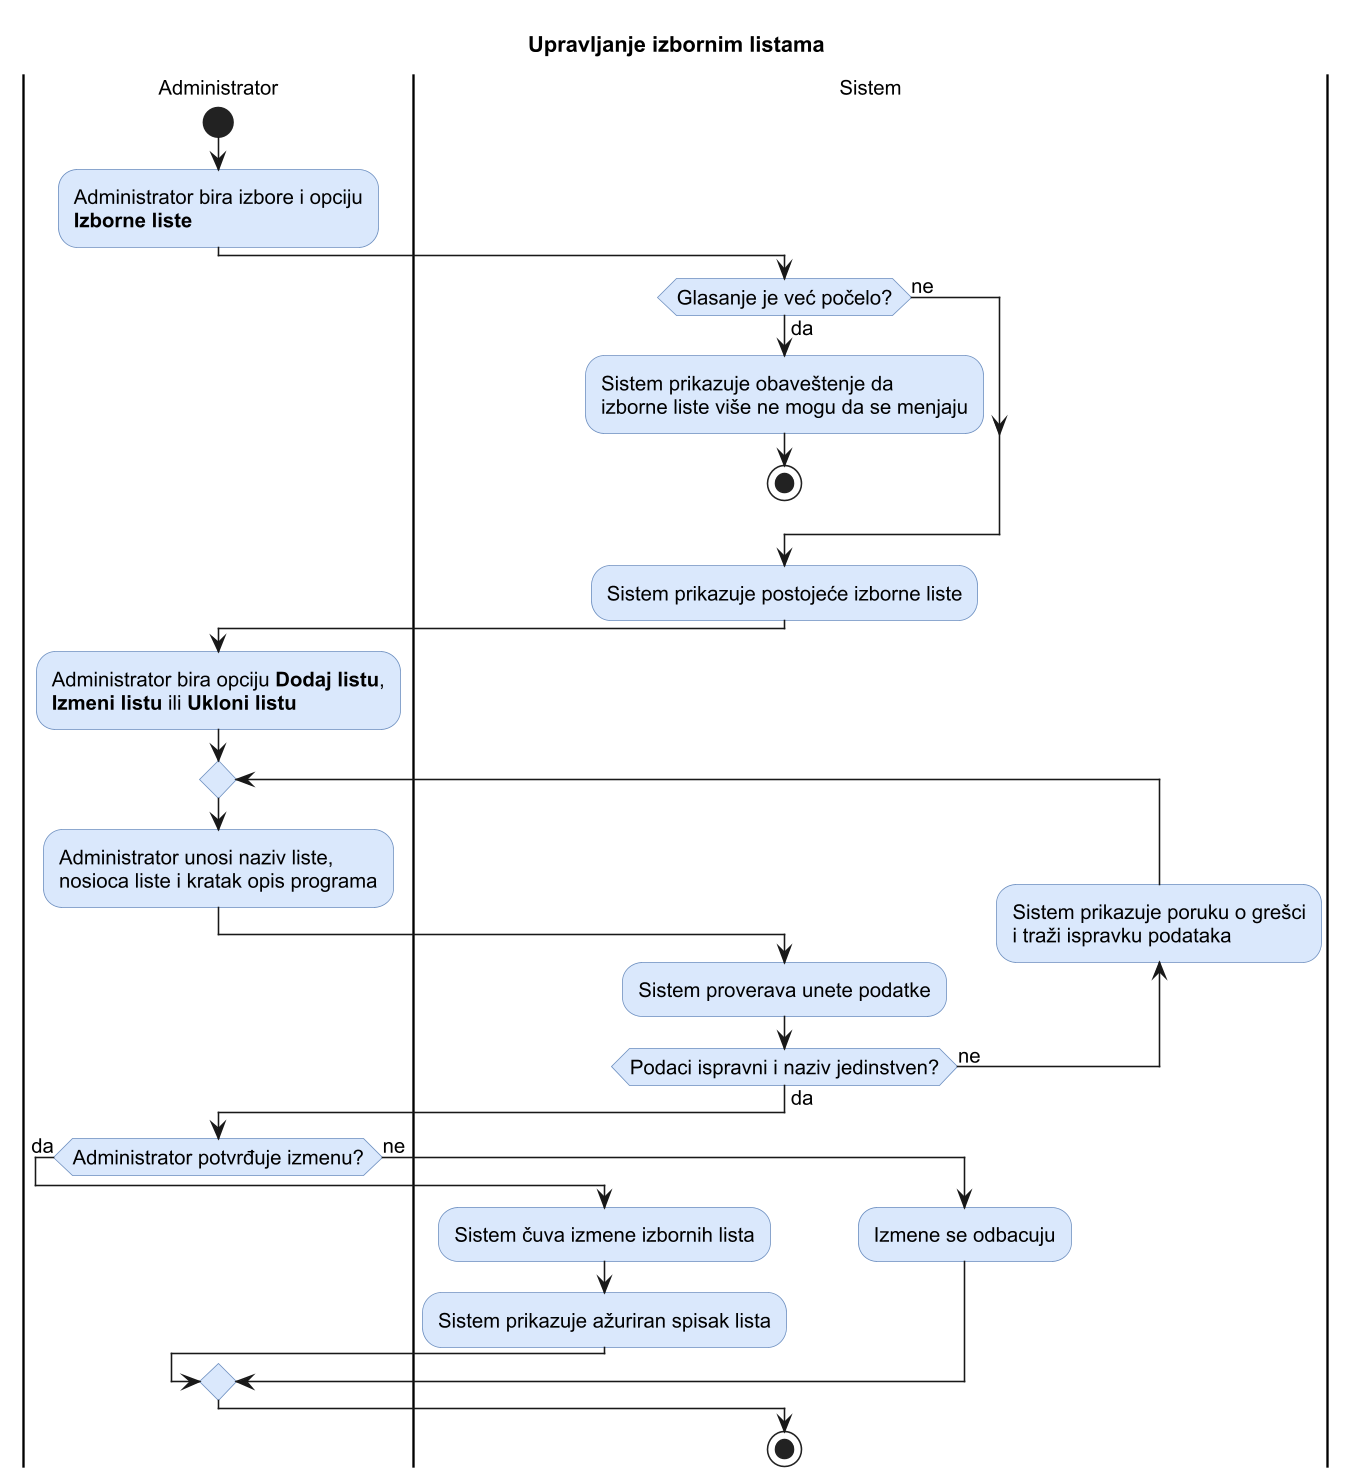
\includegraphics[width=0.85\textwidth]{aktivnosti_upravljanje_izbornim_listama.png}
    \caption{Dijagram aktivnosti: Upravljanje izbornim listama}
    \label{fig:upravljanje_izbornim_listama}
\end{figure}

\newpage
